Angel"ahnt an das  Paper \glqq From Social Media to Social Product Development: The Impact of Social Media on Co-Creation of Innovation'' \textit{(Piller et al. 2012)} werden verschiedene Methoden des Co-Creation-Prozesses beschrieben und welche Auswirkungen die wachsende Verbreitung von Social Media auf das Co-Creation hat. Co-Creation wird dabei als Weg zur Nutzung des Innovationspotentials der Konsumenten bezeichnet, in dem man sie in den firmeneigenen Innovationsprozess einbindet. Untermauert wird die theoretische Abarbeitung mit dem Thema durch 3 reale Fallbeispiele.

\subsection{Co-Creation Methoden}
Das Paper beschreibt die Kategorien Sozial Exchange und Market Exchange durch die Art und Form der Belohnung die die Konsumenten durch das Mitwirken an den jeweiligen Methoden erhalten. Sozial Exchange Methoden kennzeichnen sich dabei vor allem durch intrinsische Belohnungen wie Spa\ss{} und weniger durch extrinsische wie Geld, obwohl Anerkennung durch andere Personen oder Firmen allerdings  schon eine Rolle spielen k\"onnen. Bei Market Exchange ist es genau anders herum. Es wird aber nicht nur eine Unterteilung der Co-Creation Exchange Arten sondern auch der Art der ben"otigten Information durch das Paper vorgenommen.
Auf der einen Seite gibt es Methoden die sich mit den Bed\"urfnissen der Kunden, der sogenannten Need-Information befassen. Wenn man wei"s, was den Kunden zum Kauf motiviert, welche Vorlieben er hat, etc. kann man das Risiko einer Fehlinvestition reduzieren. Auf der anderen Seite versuchen manche Methoden das Know-How, die sogenannte Solution-Information, welche die Kunden haben, auszun\"utzen.
Laut Paper-Information, wie man eine Technologie anwendet um Kundenbed\"urfnisse in Produkte und Dienstleistungen zu verwandeln. 
 Die Methoden lassen sich durch die zwei Dimensionen anhand einer Matrix veranschaulichen. Wie in Abbildung \ref{coCreationDiagram} verdeutlicht, je nachdem was f�r eine Information ben"otigt wird, werden die entsprechenden Methoden gew"ahlt. Es wird f\"ur jedes der vier Matrixfelder eine Methode besprochen: Toolkits f\"ur User Co-Design, die Lead-User Methode, Ideation Contests und Technical Solution Contests.
\pagebreak
\begin{figure}[h!]
	\caption{Zuordnung der Co-Creation Methoden\cite{COCREATION}}
	\centering
		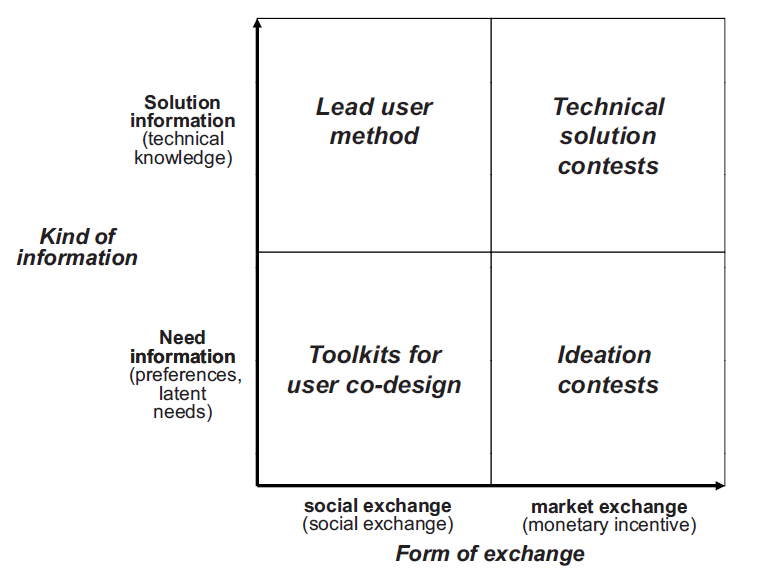
\includegraphics[scale=0.8]{figures/Co-Creation_Matrix}
	\label{coCreationDiagram}
\end{figure}
Das Aufkommen von Sozial Media ver\"andert die Methoden jedoch. Es entstehen neue M\"oglichkeiten aber auch neue Gefahren.  Au\ss{}erdem stellt das Paper die These auf, das die Einteilung der Methoden in Exchange Kategorien etwas verschwimmen werden. D.h. bei Market Exchange Methoden werden intrinsische Belohnungen eine gr\"o\ss{}ere Rolle spielen und umgekehrt bei Sozial Exchange Methoden. Als Erstes befassen wir uns mit den Methoden, die sich durch Sozial Exchange kennzeichnen.